\documentclass{article}
\usepackage[english, spanish]{babel}
\usepackage{float}
\usepackage[letterpaper, portrait, margin=2.54cm]{geometry} % Combinada y actualizada
\usepackage{graphicx}
\usepackage{lipsum}
\usepackage{amsmath,amssymb,amsthm}
\usepackage[utf8]{inputenc}
\usepackage{multirow}
\usepackage{csquotes}
\usepackage{apacite}
\usepackage{multicol}
\usepackage{parskip}
\usepackage{setspace}
\usepackage{empheq}
\usepackage{mdframed}
\usepackage{booktabs}
% \usepackage{lipsum} % Eliminado, ya cargado
% \usepackage{graphicx} % Eliminado, ya cargado
\usepackage{color}
\usepackage{psfrag}
\usepackage{pgfplots}
\usepackage{bm}
\usepackage{tocloft}
\usepackage{lscape}
\usepackage{adjustbox}
\setlength{\tabcolsep}{1.505625pt}
\renewcommand{\arraystretch}{1.2}
%%%%%%%%%%%%%%%%%%%%%%%%%%%%%%%%%%%%%%%%%%%%%%%%%%%%%%%%%%%%%%%%%%%%%%%%%%%%%%%
\definecolor{ocre}{RGB}{243,102,25}
\definecolor{mygray}{RGB}{243,243,244}
\definecolor{deepGreen}{RGB}{26,111,0}
\definecolor{shallowGreen}{RGB}{235,255,255}
\definecolor{deepBlue}{RGB}{61,124,222}
\definecolor{shallowBlue}{RGB}{235,249,255}
%%%%%%%%%%%%%%%%%%%%%%%%%%%%%%%%%%%%%%%%%%%%%%%%%%%%%%%%%%%%%%%%%%%%%%%%%%%%%%%

%%%%%%%%%%%%%%%%%%%%%%%%%% Define an orangebox command %%%%%%%%%%%%%%%%%%%%%%%%
\newcommand\orangebox[1]{\fcolorbox{ocre}{mygray}{\hspace{1em}#1\hspace{1em}}}
%%%%%%%%%%%%%%%%%%%%%%%%%%%%%%%%%%%%%%%%%%%%%%%%%%%%%%%%%%%%%%%%%%%%%%%%%%%%%%%

%%%%%%%%%%%%%%%%%%%%%%%%%%%% English Environments %%%%%%%%%%%%%%%%%%%%%%%%%%%%%
\newtheoremstyle{mytheoremstyle}{3pt}{3pt}{\normalfont}{0cm}{\rmfamily\bfseries}{}{1em}{{\color{black}\thmname{#1}~\thmnumber{#2}}\thmnote{\,--\,#3}}
\newtheoremstyle{myproblemstyle}{3pt}{3pt}{\normalfont}{0cm}{\rmfamily\bfseries}{}{1em}{{\color{black}\thmname{#1}~\thmnumber{#2}}\thmnote{\,--\,#3}}
\theoremstyle{mytheoremstyle}
\newmdtheoremenv[linewidth=1pt,backgroundcolor=shallowGreen,linecolor=deepGreen,leftmargin=0pt,innerleftmargin=20pt,innerrightmargin=20pt,]{theorem}{Theorem}[section]
\theoremstyle{mytheoremstyle}
\newmdtheoremenv[linewidth=1pt,backgroundcolor=shallowBlue,linecolor=deepBlue,leftmargin=0pt,innerleftmargin=20pt,innerrightmargin=20pt,]{definition}{Definition}[section]
\theoremstyle{myproblemstyle}
\newmdtheoremenv[linecolor=black,leftmargin=0pt,innerleftmargin=10pt,innerrightmargin=10pt,]{problem}{Problem}[section]
%%%%%%%%%%%%%%%%%%%%%%%%%%%%%%%%%%%%%%%%%%%%%%%%%%%%%%%%%%%%%%%%%%%%%%%%%%%%%%%

%%%%%%%%%%%%%%%%%%%%%%%%%%%%%%% Plotting Settings %%%%%%%%%%%%%%%%%%%%%%%%%%%%%
\usepgfplotslibrary{colorbrewer}
\pgfplotsset{width=8cm,compat=1.18} % Unificado y compatibilidad actualizada
%%%%%%%%%%%%%%%%%%%%%%%%%%%%%%%%%%%%%%%%%%%%%%%%%%%%%%%%%%%%%%%%%%%%%%%%%%%%%%%

%%%%%%%%%%%%%%%%%%%%%%%%%%%%%%% Title & Author %%%%%%%%%%%%%%%%%%%%%%%%%%%%%%%%
\author{Gustavo Vergara}
%%%%%%%%%%%%%%%%%%%%%%%%%%%%%%%%%%%%%%%%%%%%%%%%%%%%%%%%%%%%%%%%%%%%%%%%%%%%%%%

\begin{document}
% \pgfplotsset{compat=1.18} % Movido al preámbulo
\setstretch{2}

\begin{titlepage}
    \centering
    \vspace{2.5cm}
    {\scshape \Large ESTUDIO DEL COMPORTAMIENTO TÉRMICO DE UN ROTOR\par} % Texto añadido/modificado
    \vspace{5cm}
    % \textbf\large\scshape{\par} % Esta línea estaba vacía, puedes añadir texto o eliminarla
    \vspace{0.5cm}
    {\Large VERGARA PAREJA GUSTAVO\par}
    \vspace{5cm}
    {\scshape\Large Ávila Díaz Cesar Iván\par}
    \vspace{0.3cm}
    {\scshape\Large MEF COMPUTACIONAL \par}
    \vspace{0.3cm}
    {\scshape\Large Universidad de Córdoba\par}
    \vspace{0.3cm}
    {\Large 31 de Mayo de 2025 \par}
\end{titlepage}
\tableofcontents
\newpage
\section{Introducción}

    A continuación realizaremos el estudio del comportamiento térmico de un rotor a causa de la fricción de los cojinetes y el flujo de calor del lubricante. Para ello, utilizaremos el software COMSOL Multiphysics, que nos permitirá modelar y simular el comportamiento térmico del rotor bajo estas condiciones de operación.
\section{Definición del modelo}
  \begin{itemize}
    \item \textbf{Transferencia de Calor en las Películas de Lubricante (Heat Transfer in Films):} Modela el flujo de calor debido a la convección entre el lubricante y las superficies de contacto del rotor y el casquillo.
    \item \textbf{Rodamientos Hidrodinámicos (Hydrodynamic Bearings):} Simula la distribución de presión en la película de lubricante y la disipación de calor debido a la viscosidad del lubricante.
    \item \textbf{Mecánica de Sólidos (Solid Mechanics):} Calcula las deformaciones y tensiones térmicas en el rotor y las carcasas debido al calentamiento no uniforme del sistema.
    \item \textbf{Expansión Térmica (Thermal Expansion):} Transfiere la temperatura de las superficies de contacto del lubricante a las superficies sólidas del rotor y las carcasas para computar la expansión térmica y las tensiones asociadas.
  \end{itemize}
          \section{Implementación en COMSOL}
          Para implementar el modelo en COMSOL, se debe crear un nuevo modelo y seleccionar los módulos presentados a continuación:
\subsection{Definimos los estudios a realizar}
  \begin{figure}[H]
              \centering
              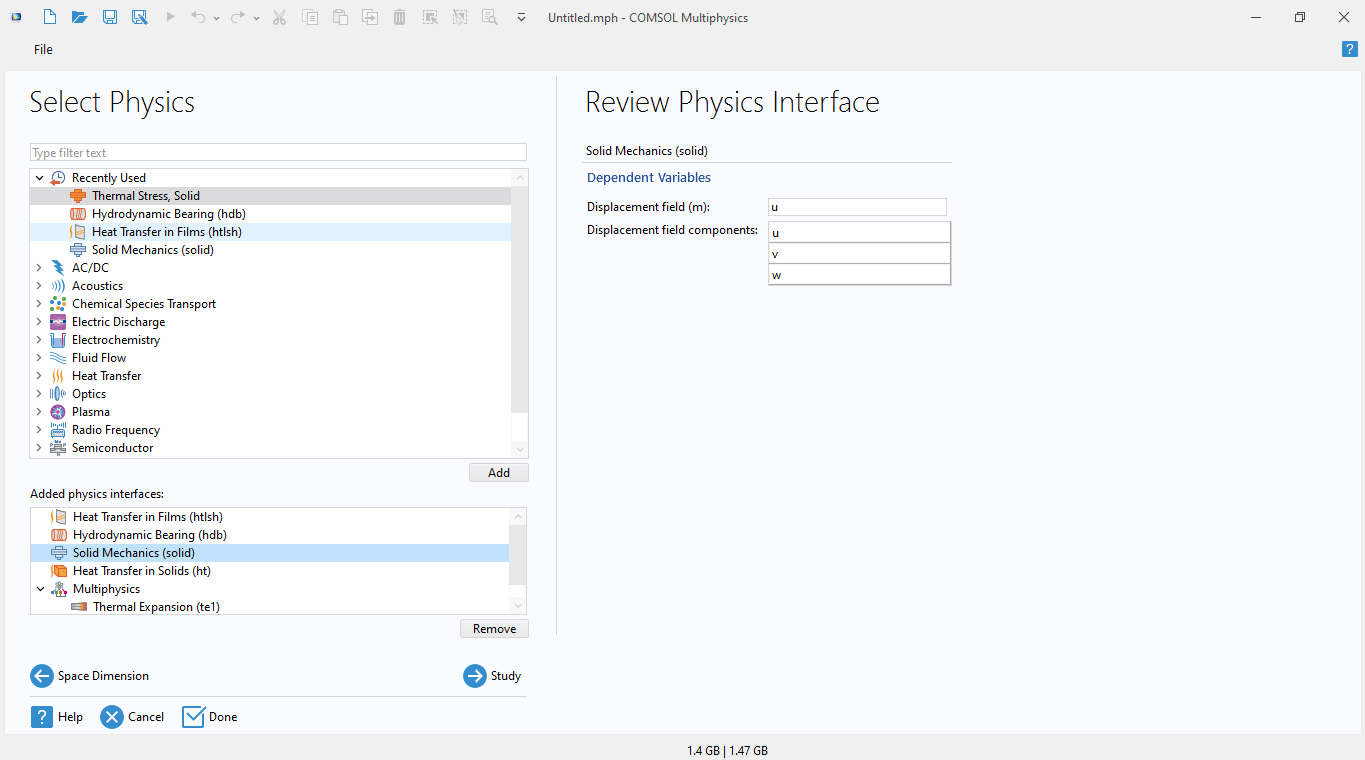
\includegraphics[width=0.9\textwidth]{estu.png}
              \caption{Estudios}
              \label{fig:comsol_estudios}
            \end{figure}
\subsection{Importamos la geometría a estudiar}
\begin{figure}[H]
              \centering
              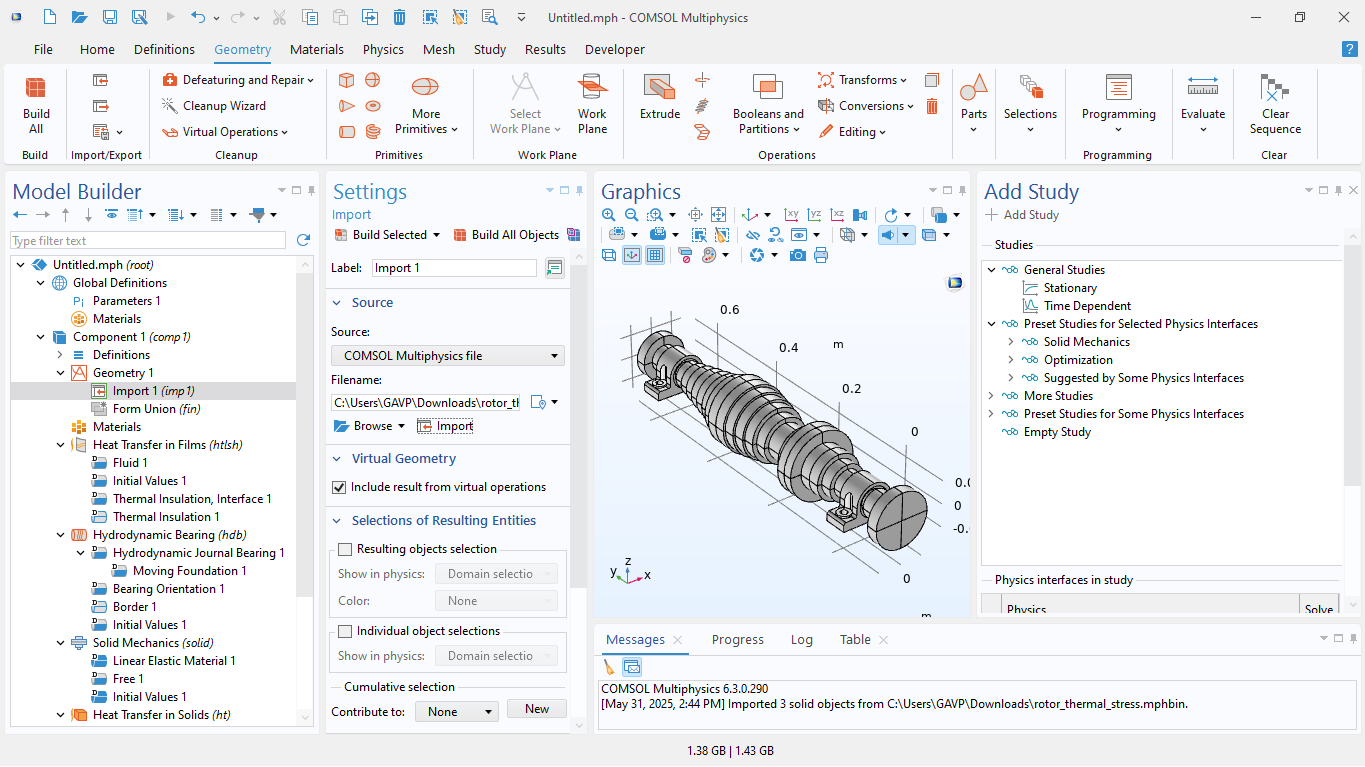
\includegraphics[width=0.9\textwidth]{geom.png}
              \caption{Rotor}
              \label{fig:comsol_geometria_rotor} % Etiqueta renombrada para mayor claridad
            \end{figure}

            \subsection{Creamos las uniones}
            \begin{figure}[H]
              \centering
              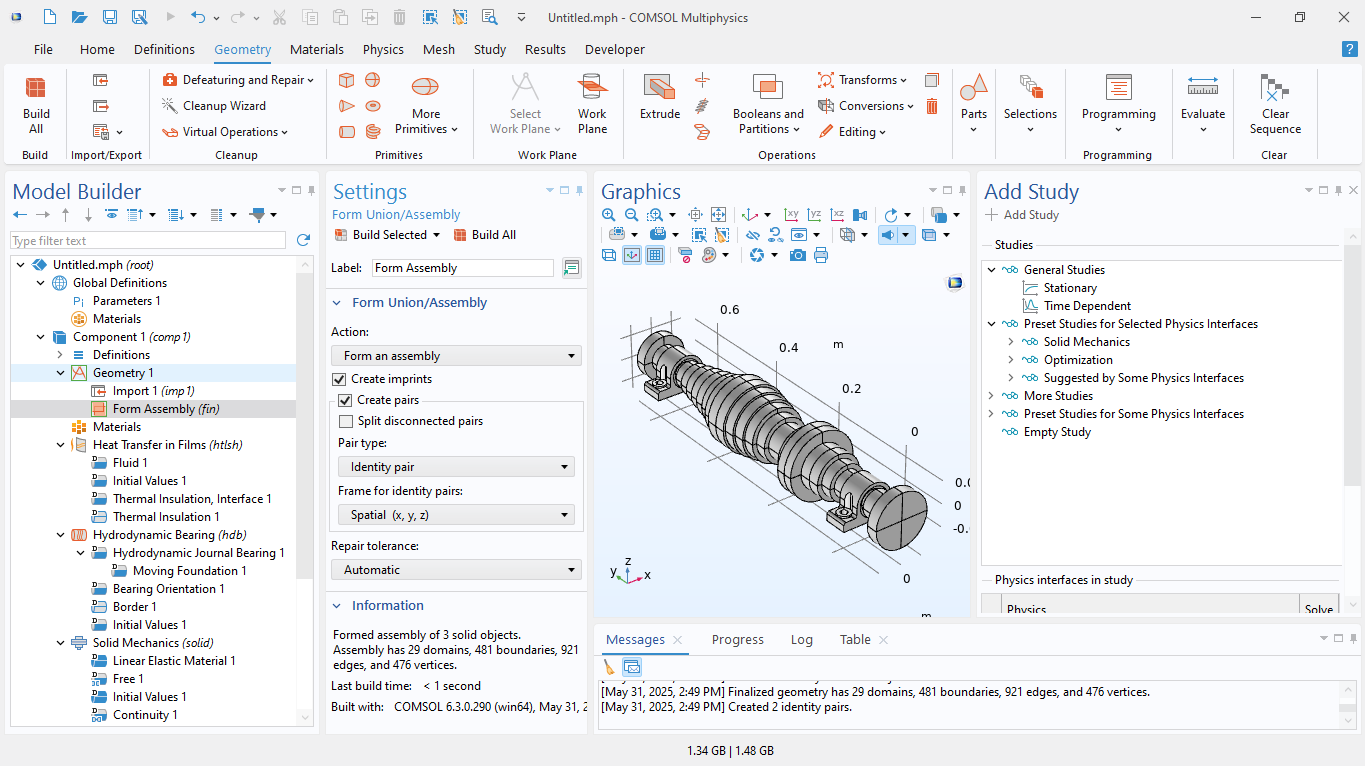
\includegraphics[width=0.9\textwidth]{uniones.png}
              \caption{Uniones}
              \label{fig:comsol_uniones} % Etiqueta renombrada para mayor claridad
            \end{figure}

            \subsection{Definimos los elementos y variables}
            \begin{figure}[H]
              \centering
              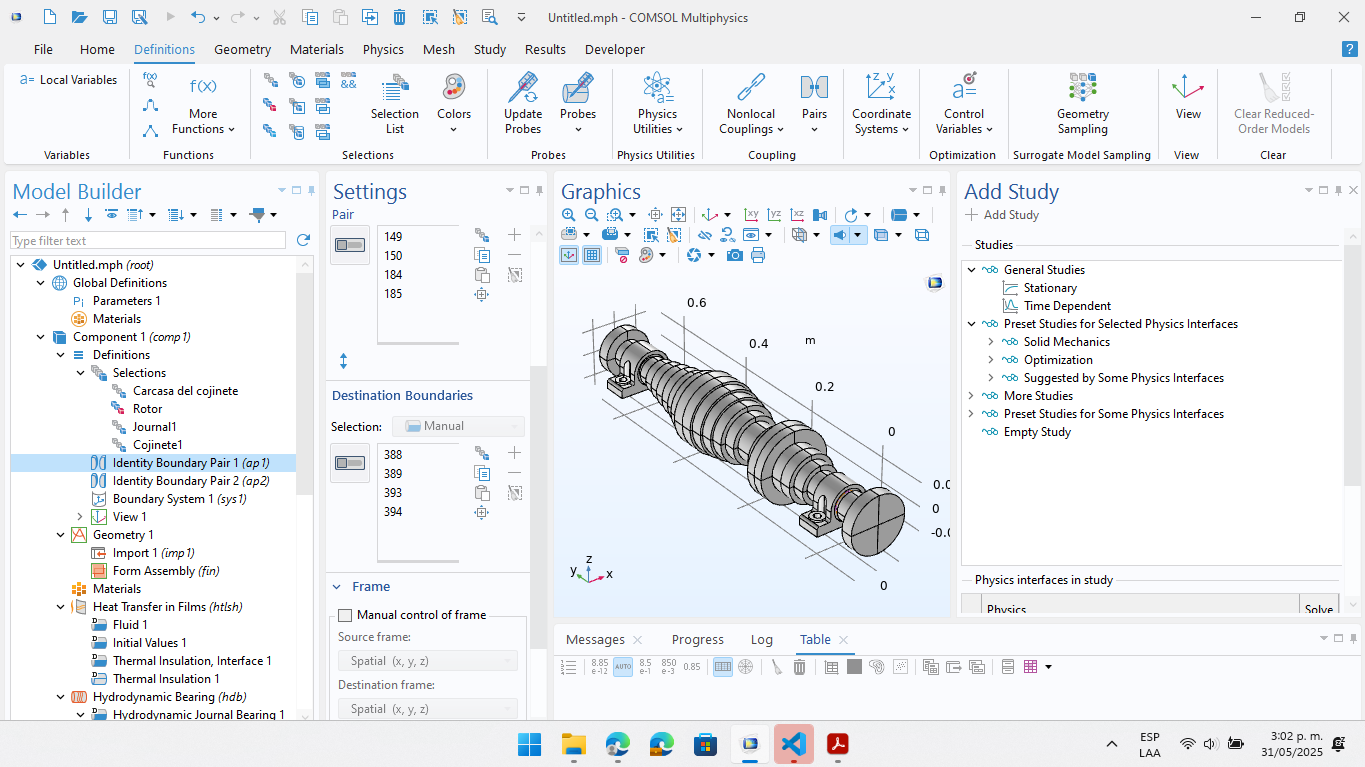
\includegraphics[width=0.9\textwidth]{def_elem.png}
              \caption{Definición de elementos}
              \label{fig:comsol_parametros_geometria}
            \end{figure} % Fin de la figura anterior, se desanidaron las siguientes

            \begin{figure}[H] % Figura desanidada
              \centering
              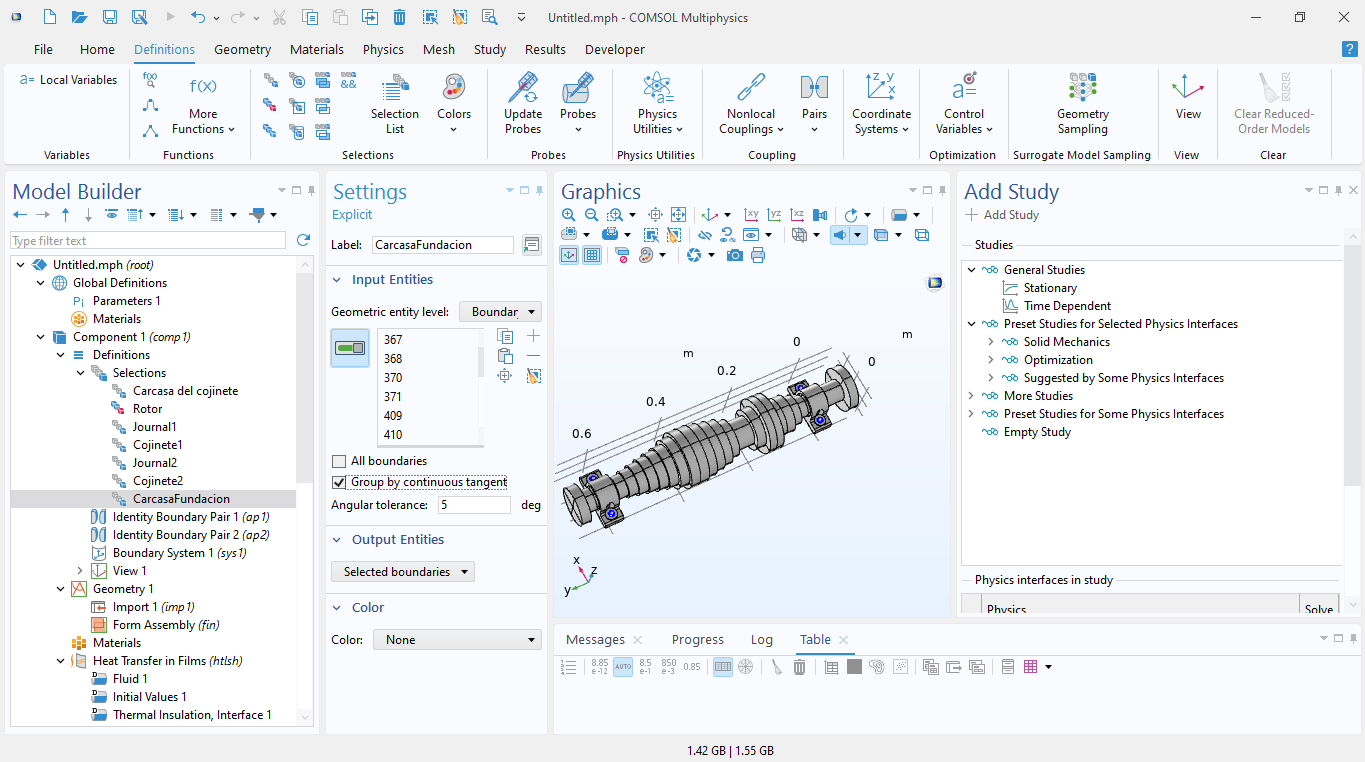
\includegraphics[width=0.9\textwidth]{carcas.png}
              \caption{Definición de carcasas} % Caption añadido/corregido
              \label{fig:comsol_definicion_carcasas} % Etiqueta renombrada
            \end{figure}

            \begin{figure}[H] % Figura desanidada
              \centering
              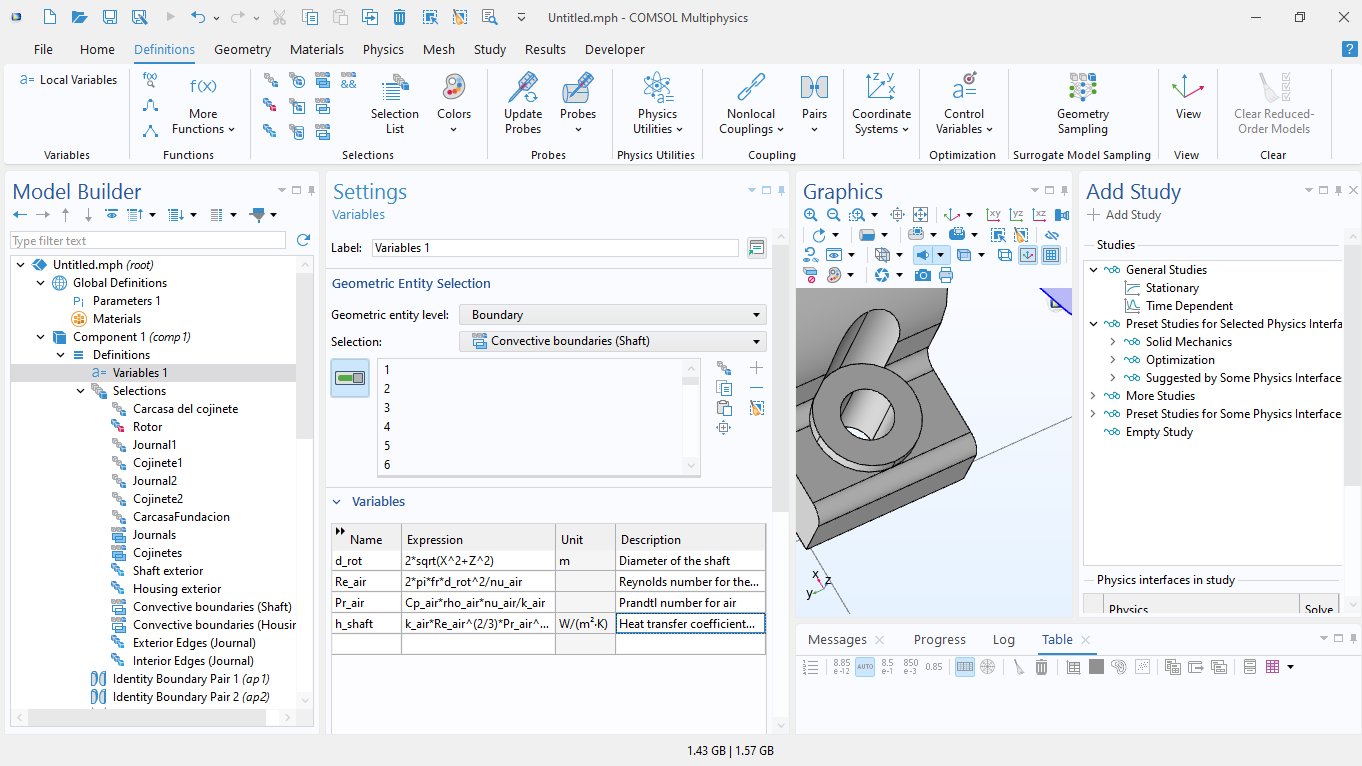
\includegraphics[width=0.9\textwidth]{vari.png}
              \caption{Variables}
              \label{fig:comsol_variables_definicion} % Etiqueta renombrada
            \end{figure}
            \subsection{Agregamos los materiales}
               \begin{figure}[H]
              \centering
              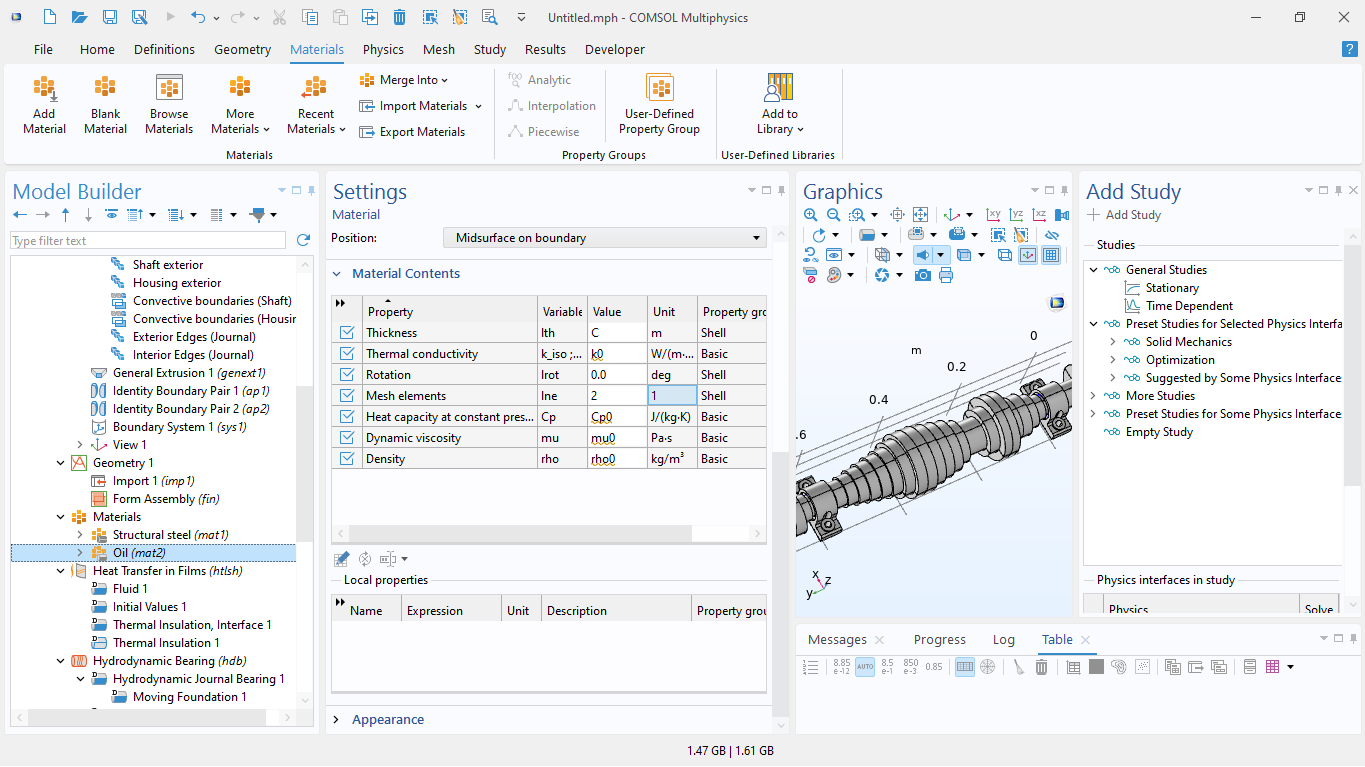
\includegraphics[width=0.9\textwidth]{mat2.png}
              \caption{Oil}
              \label{fig:comsol_material_oil} % Etiqueta renombrada
            \end{figure}

  \subsection{Definimos fenómeno de transferencia de calor}
            \begin{figure}[H]
              \centering
              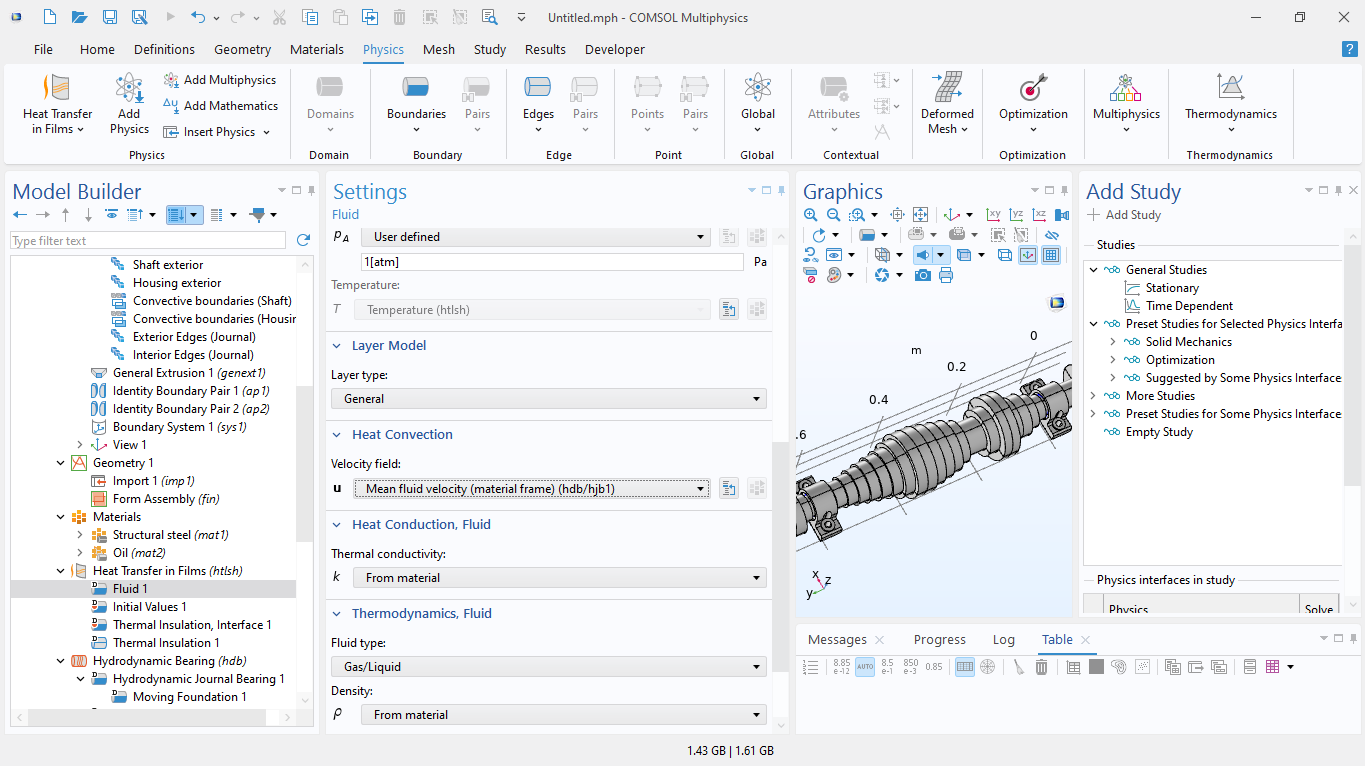
\includegraphics[width=0.9\textwidth]{fen.png}
              \caption{Fenómeno de transferencia de calor}
              \label{fig:comsol_fen_transf_calor_1} % Etiqueta corregida
            \end{figure}
            \begin{figure}[H]
              \centering
              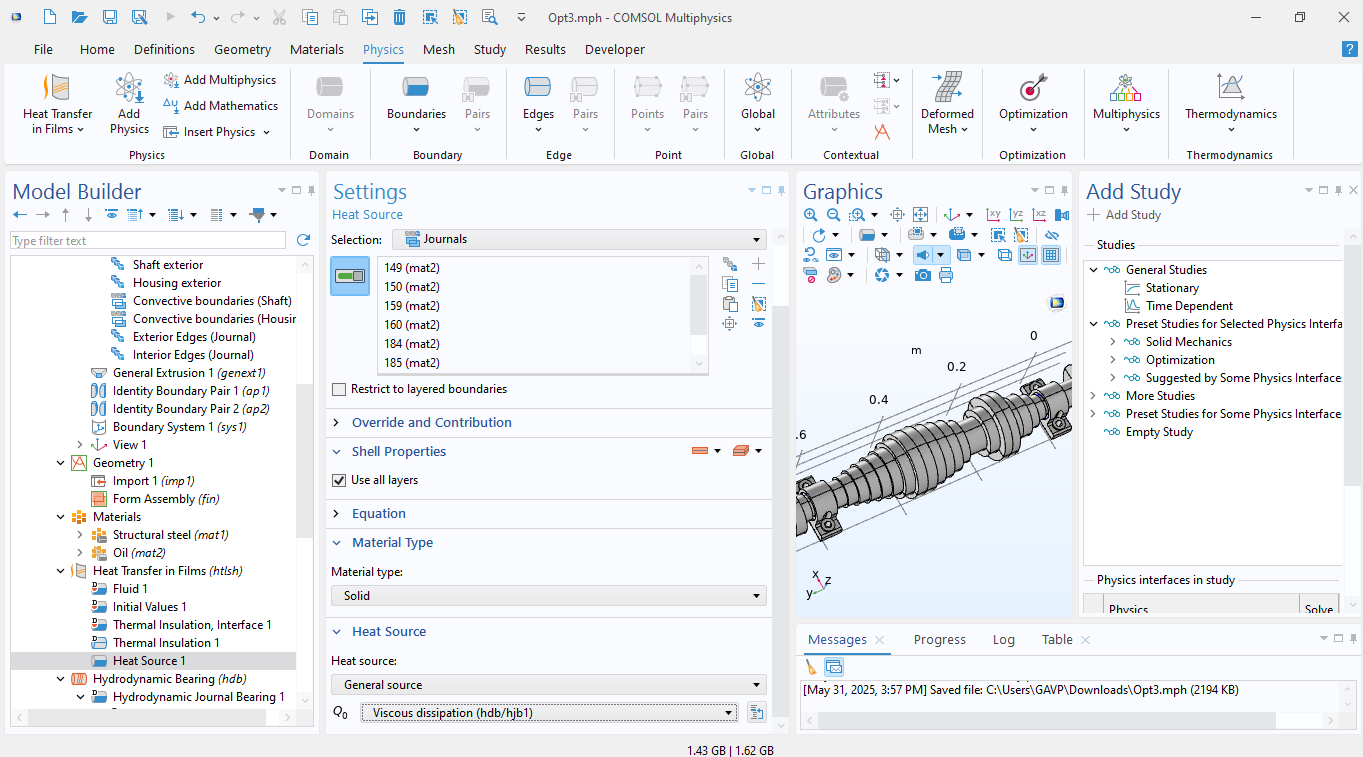
\includegraphics[width=0.9\textwidth]{fen2.png}
              \caption{Fenómeno de transferencia de calor 2}
              \label{fig:comsol_fen_transf_calor_2} % Etiqueta corregida
            \end{figure}
     \begin{figure}[H]
              \centering
              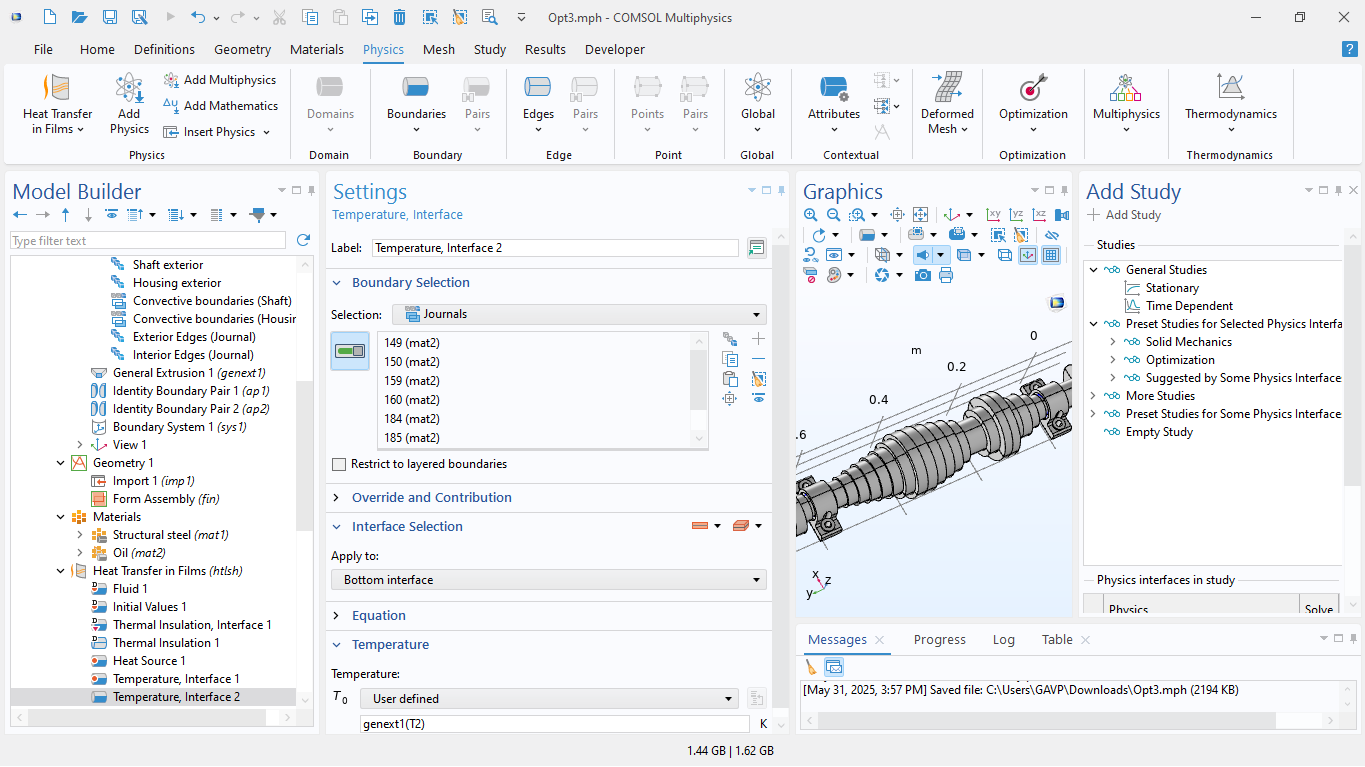
\includegraphics[width=0.9\textwidth]{fen3.png}
              \caption{Fenómeno de transferencia de calor 3}
              \label{fig:comsol_fen_transf_calor_3} % Etiqueta corregida
            \end{figure}

             \subsection{Definimos fenómeno hidrodinámico en los cojinetes}
            \begin{figure}[H]
              \centering
              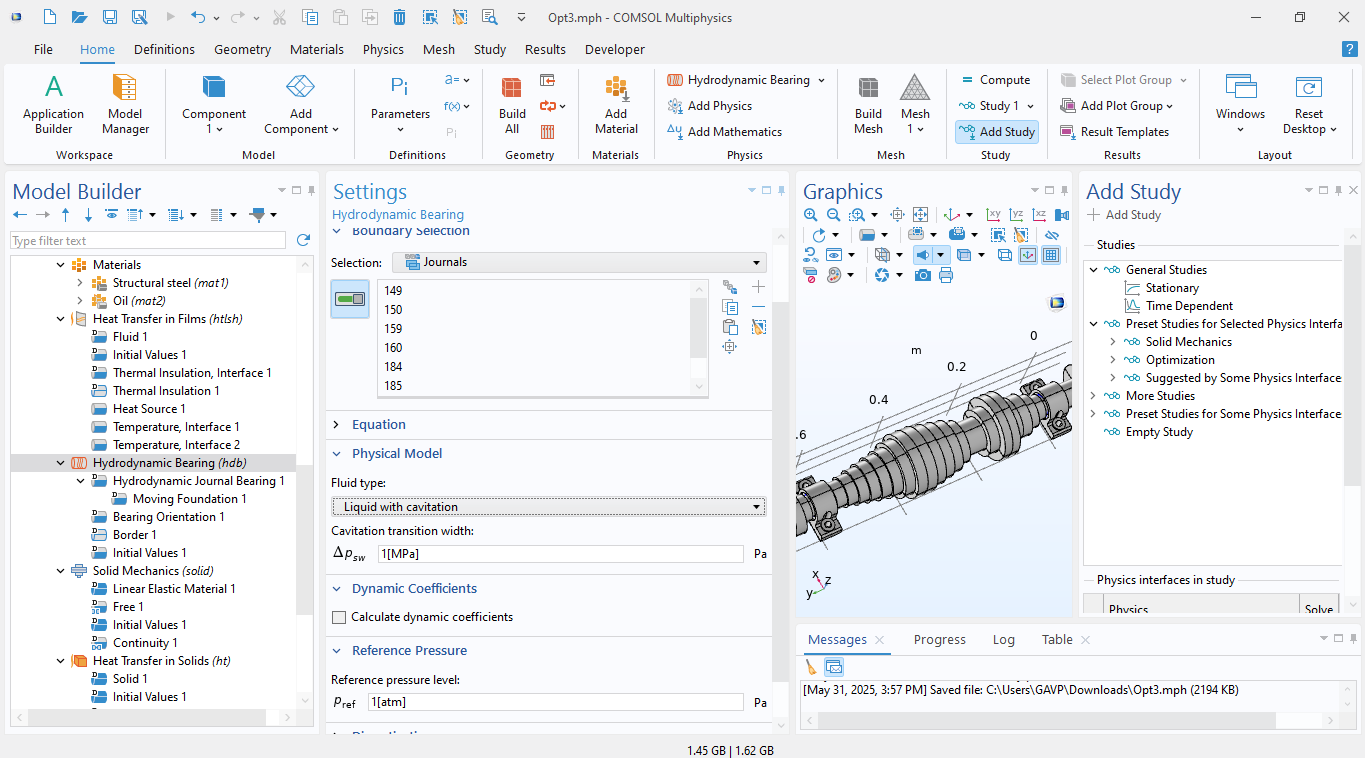
\includegraphics[width=0.9\textwidth]{fen4.png}
              \caption{Fenómeno hidrodinámico}
              \label{fig:comsol_fen_hidrodinamico_1} % Etiqueta corregida
            \end{figure}

             \begin{figure}[H]
              \centering
              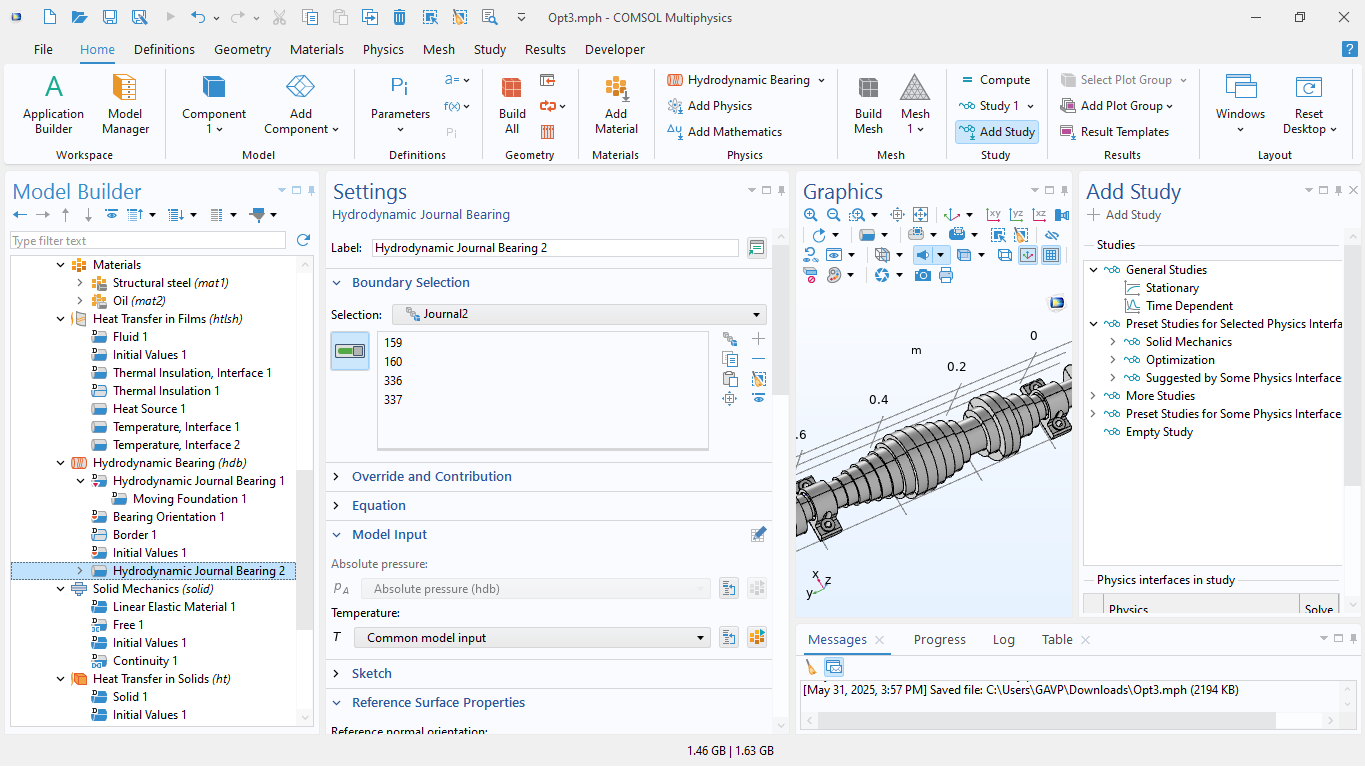
\includegraphics[width=0.9\textwidth]{fen5.png}
              \caption{Fenómeno hidrodinámico 2}
              \label{fig:comsol_fen_hidrodinamico_2} % Etiqueta corregida
            \end{figure}

             \begin{figure}[H]
              \centering
              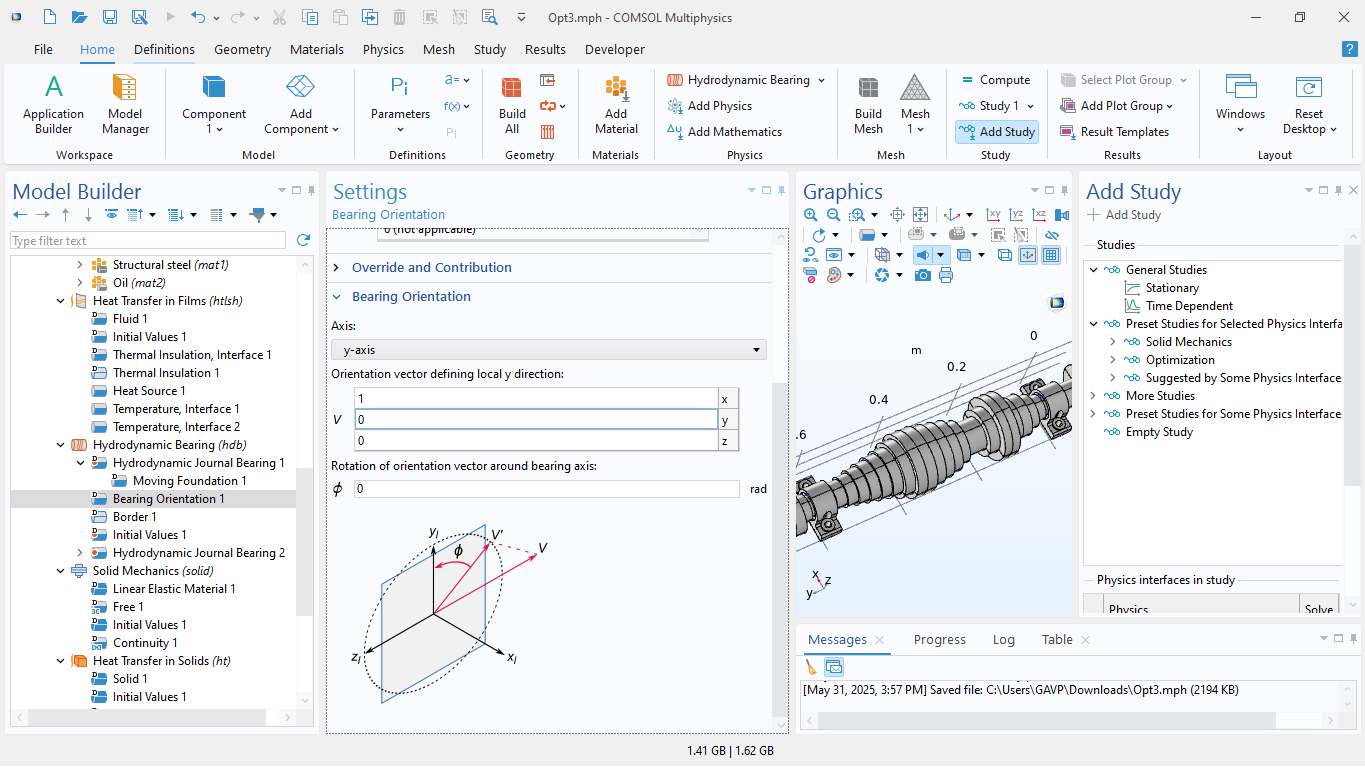
\includegraphics[width=0.9\textwidth]{ori.png}
              \caption{Fenómeno hidrodinámico 3 - Orientación del cojinete}
              \label{fig:comsol_fen_hidrodinamico_orientacion} % Etiqueta corregida
            \end{figure}

            \subsection{Definimos las condiciones de frontera y cargas}
             \begin{figure}[H]
              \centering
              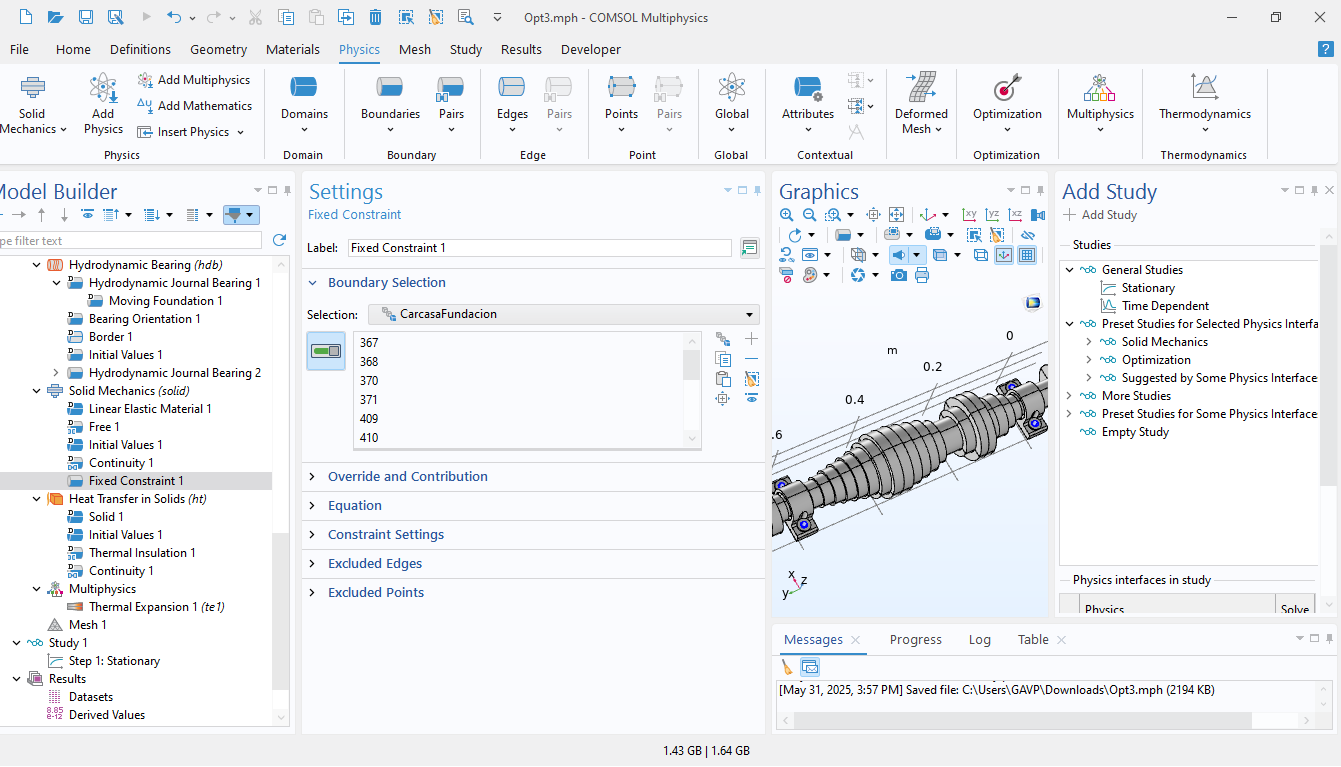
\includegraphics[width=0.9\textwidth]{restriccion1.png}
              \caption{Fijo1}
              \label{fig:comsol_cond_fijo1} % Etiqueta corregida
            \end{figure}

             \begin{figure}[H]
              \centering
              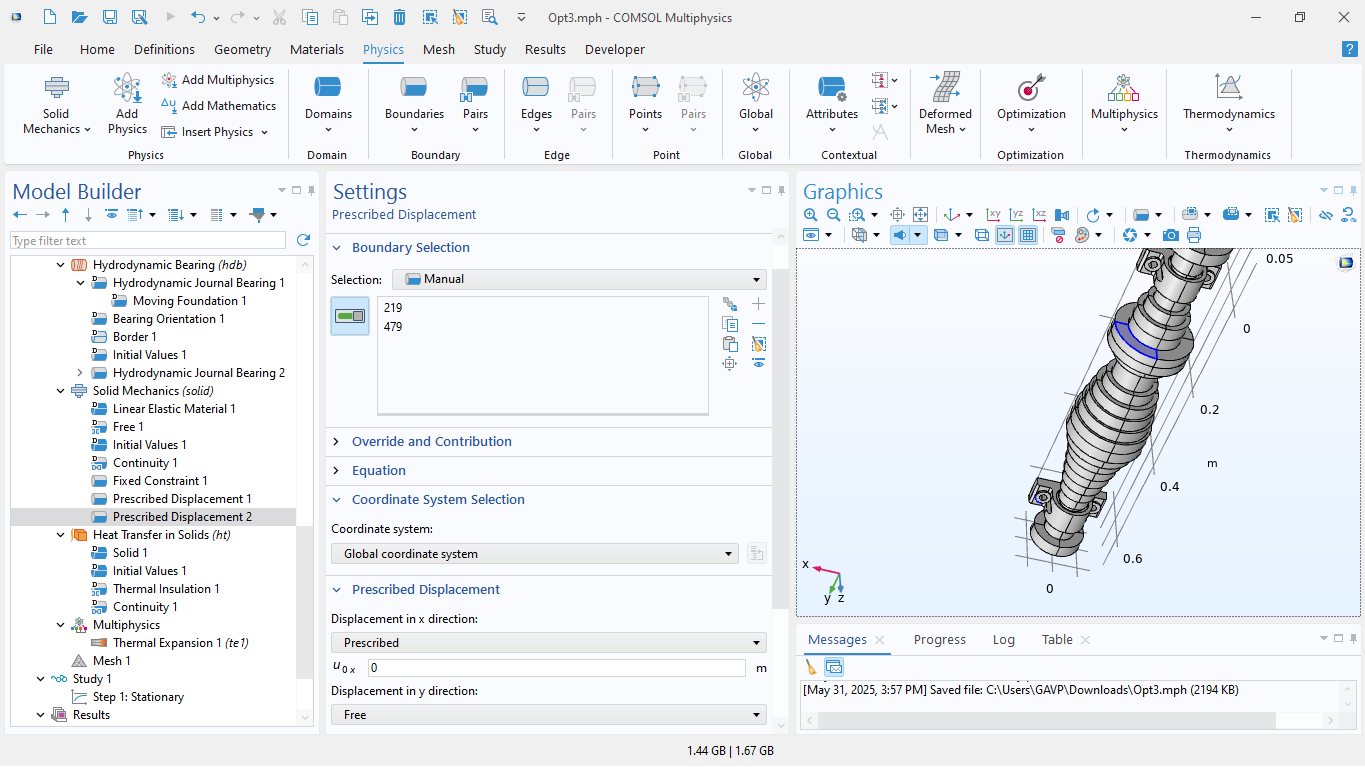
\includegraphics[width=0.9\textwidth]{dis1.png}
              \caption{Desplazamientos definidos}
              \label{fig:comsol_cond_desplazamientos} % Etiqueta corregida
            \end{figure}

            \subsection{Definimos transferencia de calor en sólidos}
             \begin{figure}[H]
              \centering
              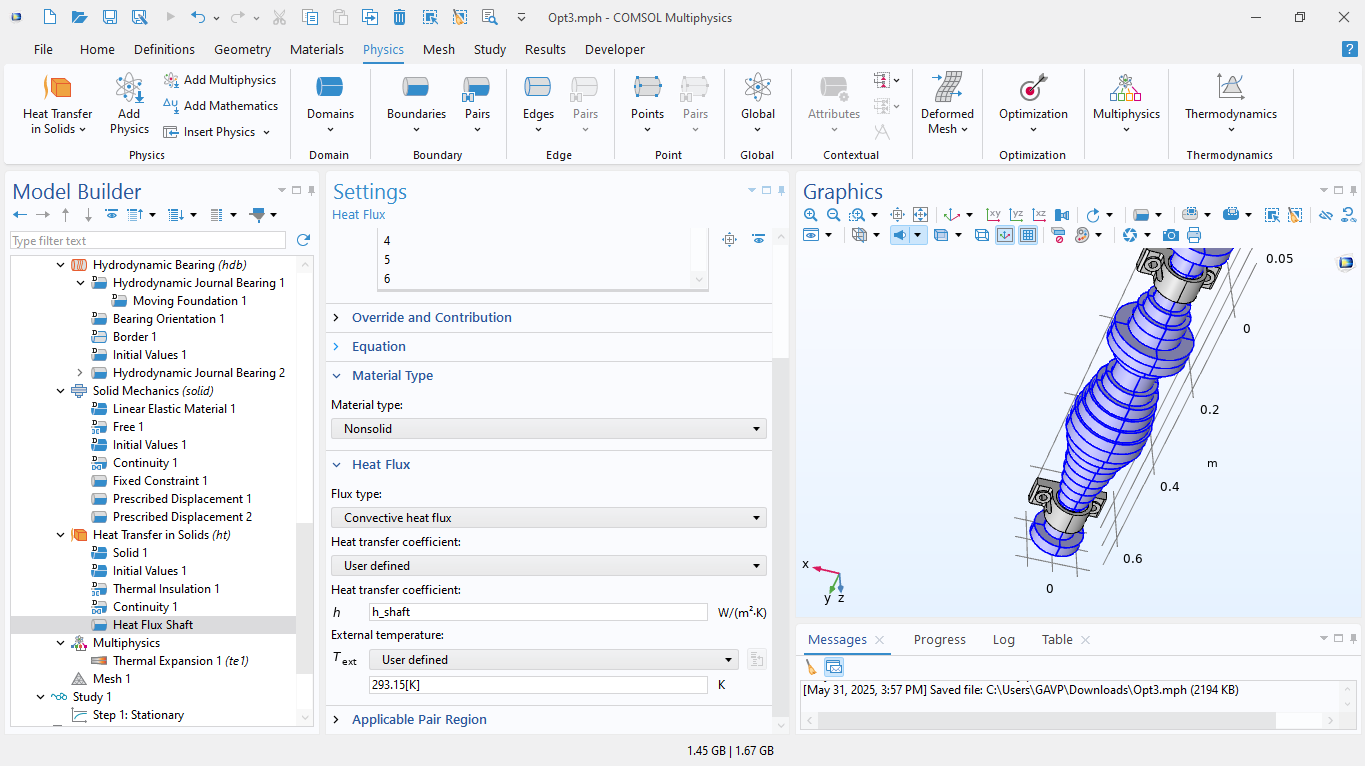
\includegraphics[width=0.9\textwidth]{htfluxeje.png}
              \caption{Flujo de calor sobre el eje}
              \label{fig:comsol_flujo_calor_eje_img} % Etiqueta corregida
            \end{figure}

             \begin{figure}[H]
              \centering
              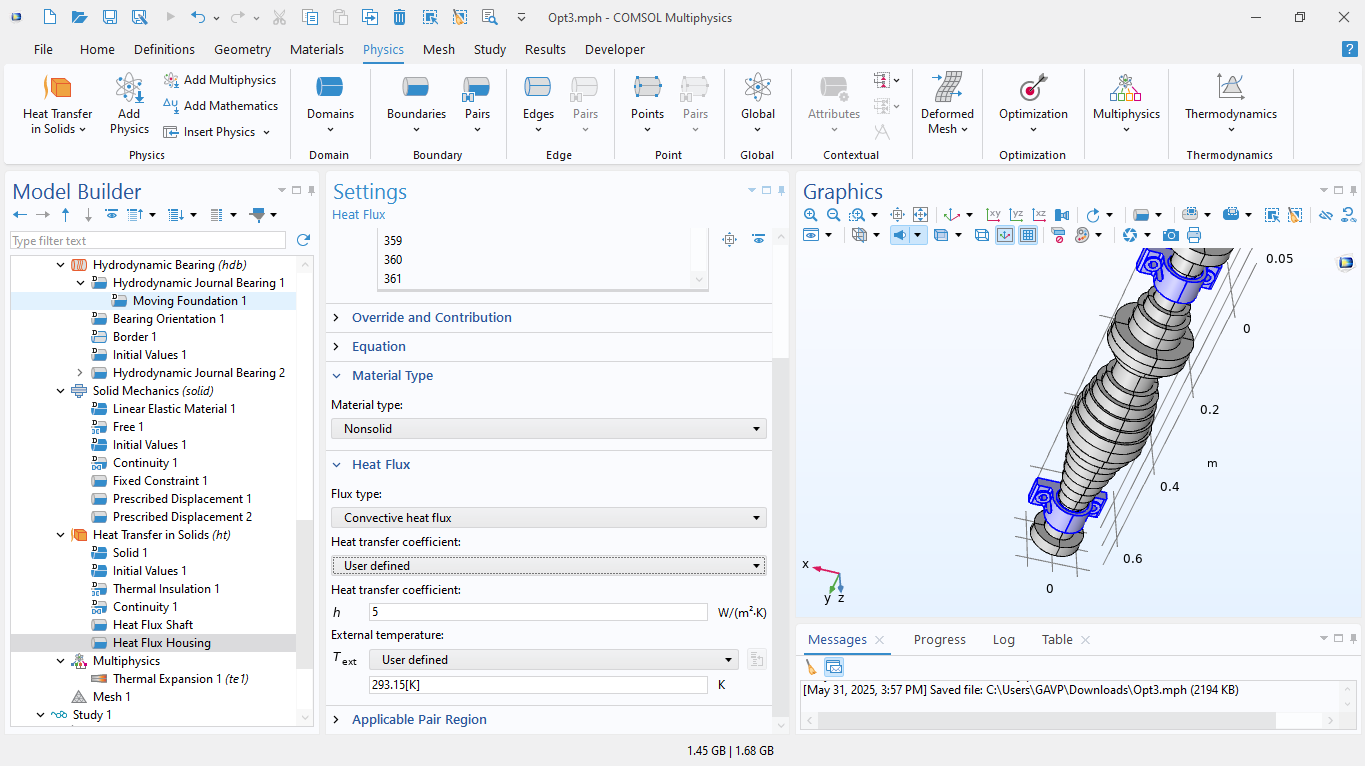
\includegraphics[width=0.9\textwidth]{htflhous.png}
              \caption{Flujo de calor sobre las carcasas}
              \label{fig:comsol_flujo_calor_carcasas}
            \end{figure}

            \subsection{Definimos la malla}
             \begin{figure}[H]
              \centering
              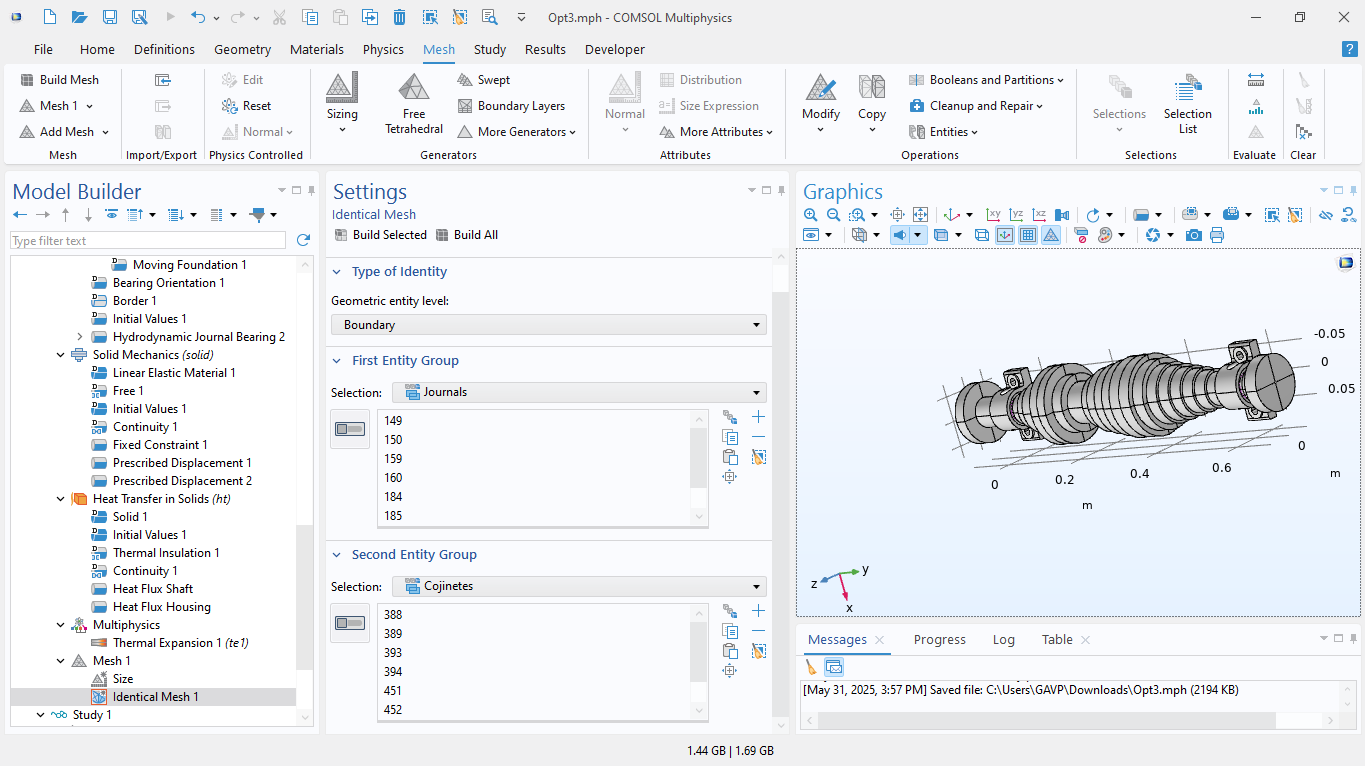
\includegraphics[width=0.9\textwidth]{id1.png}
              \caption{Malla idéntica para Journals and Bearings}
              \label{fig:comsol_malla_identica_journals_bearings} % Etiqueta corregida
            \end{figure}
             \begin{figure}[H]
              \centering
              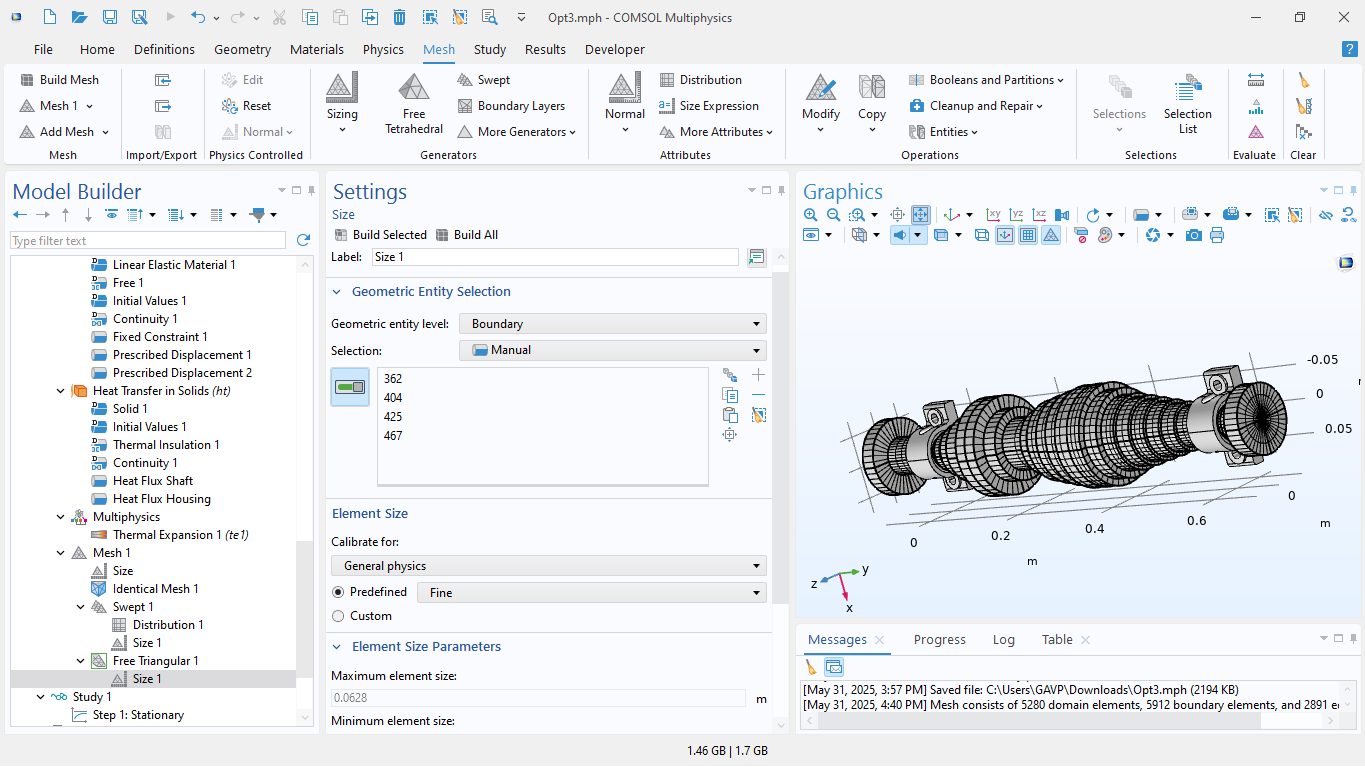
\includegraphics[width=0.9\textwidth]{mesg.png}
              \caption{Malla finalizada}
              \label{fig:comsol_malla_finalizada_img} % Etiqueta corregida
            \end{figure}

    \subsection{Ejecución del estudio}
             \begin{figure}[H]
              \centering
              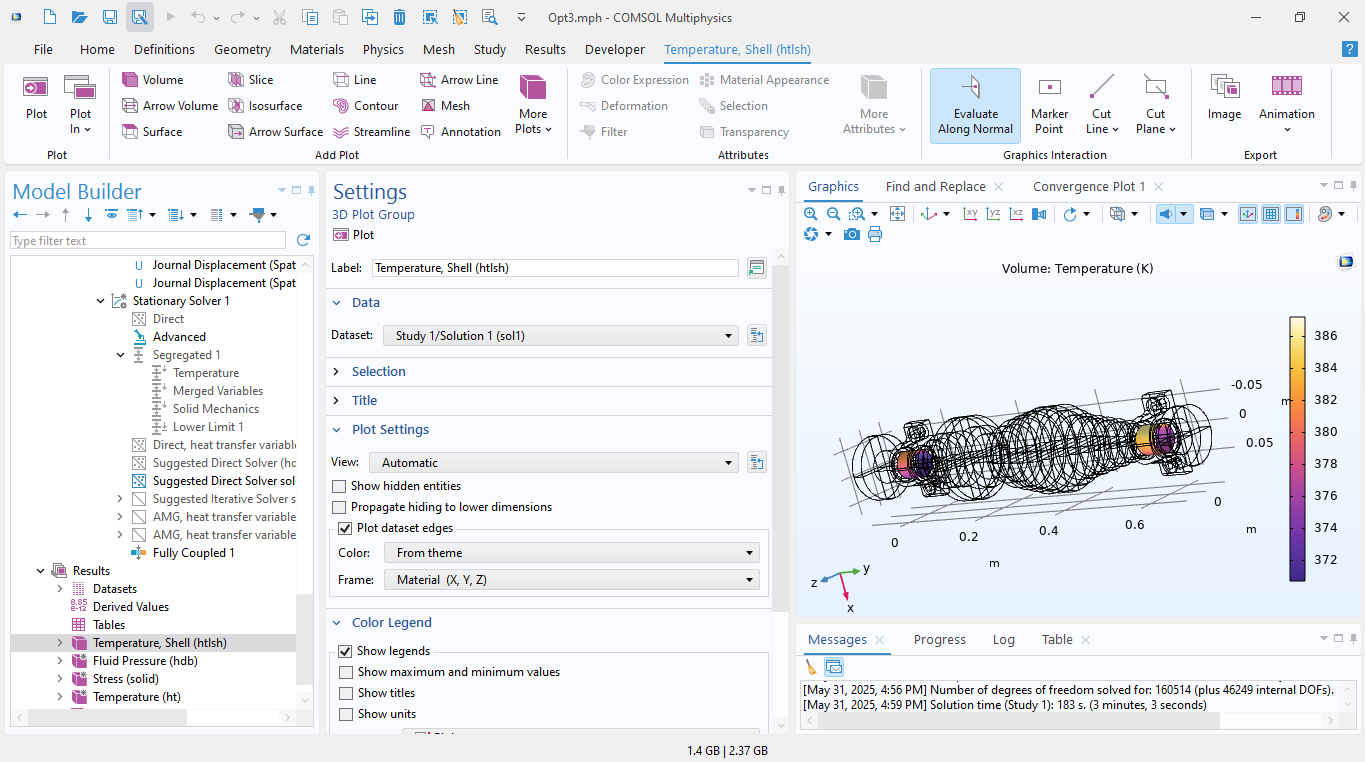
\includegraphics[width=0.9\textwidth]{comp1.png}
              \caption{Estudio computado}
              \label{fig:comsol_estudio_computado_img} % Etiqueta corregida
            \end{figure}

            \section{Resultados}
             \begin{figure}[H]
              \centering
              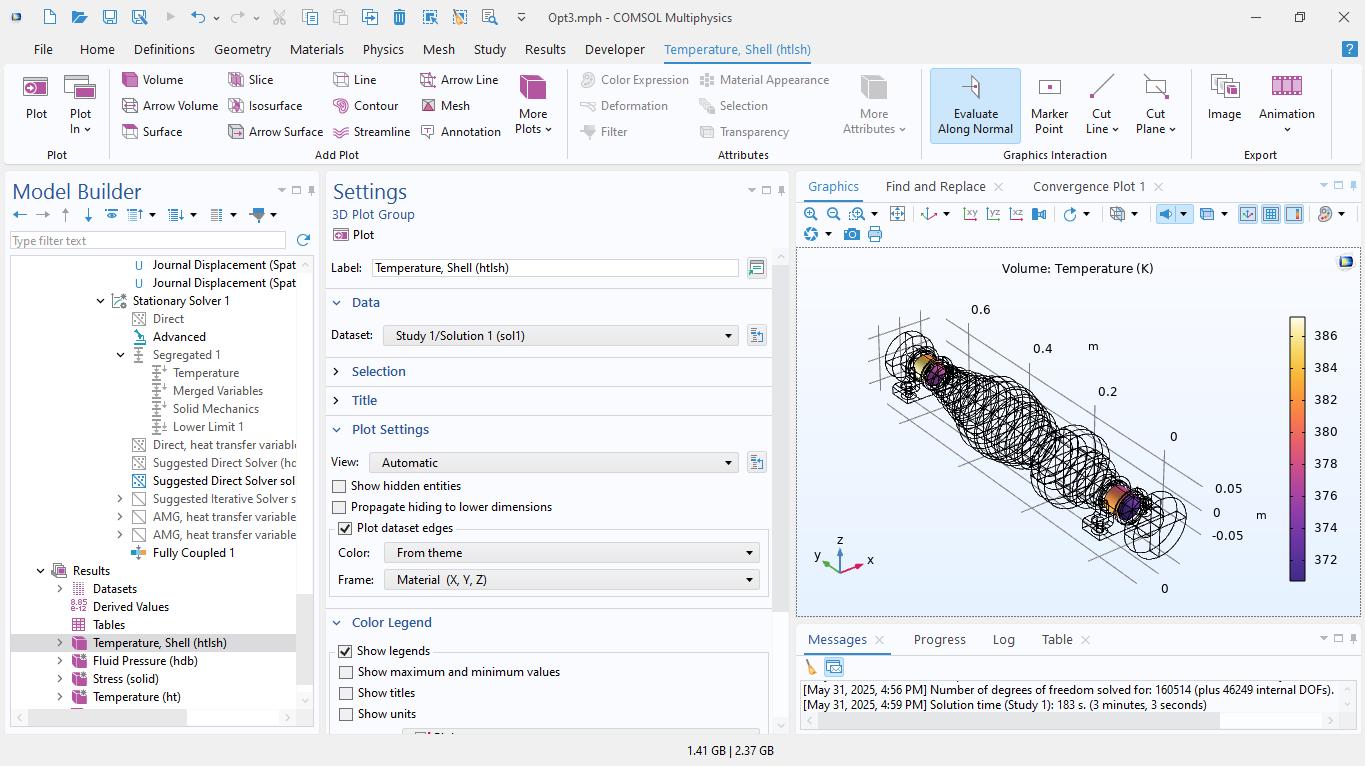
\includegraphics[width=0.9\textwidth]{temp_lubricant.png}
              \caption{Temperatura del lubricante}
              \label{fig:comsol_temp_lubricante}
            \end{figure}

            \begin{itemize}
              \item \textbf{Perfil de Temperatura:} La distribución de temperatura en el lubricante, el rotor y las carcasas muestra cómo el calor se disipa desde los rodamientos hacia el entorno.
               \end{itemize}
            \begin{figure}[H]
              \centering
              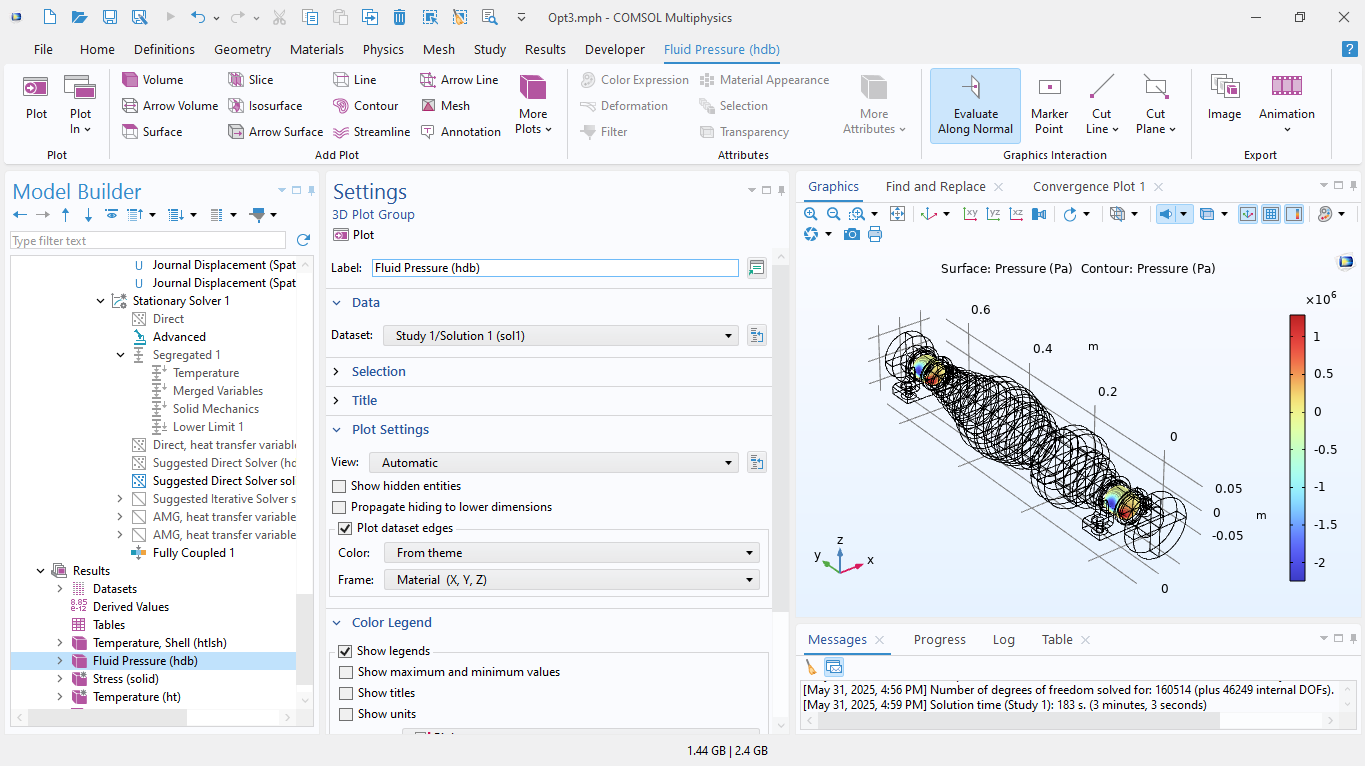
\includegraphics[width=0.9\textwidth]{fluid_pressure.png}
              \caption{Presión del fluido}
              \label{fig:comsol_presion_fluido}
            \end{figure}

            \begin{itemize}
             \item \textbf{Distribución de la Presión en los Rodamientos:} Se observó que la presión máxima se localiza en la parte inferior del rodamiento.
               \end{itemize}
             \begin{figure}[H]
              \centering
              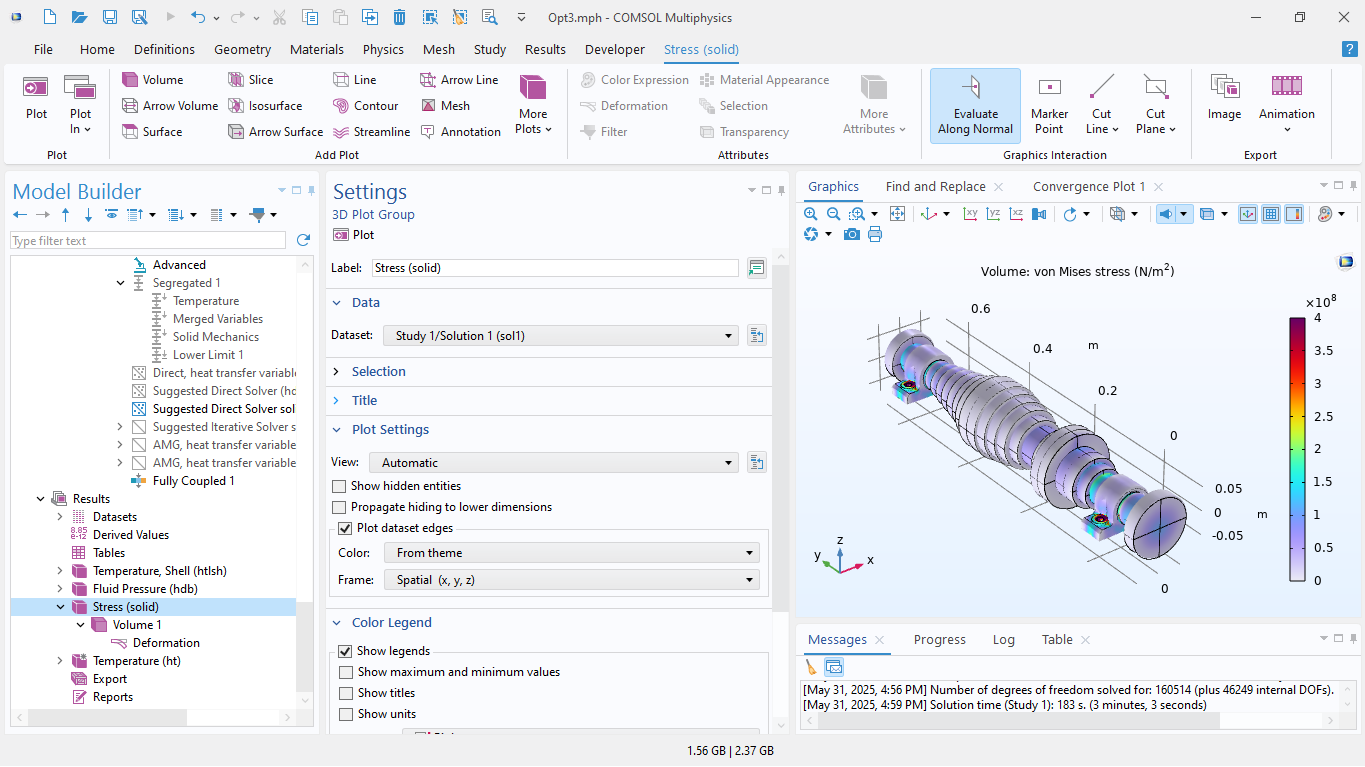
\includegraphics[width=0.9\textwidth]{Stress+Deformation.png}
              \caption{Esfuerzo y deformación}
              \label{fig:comsol_esfuerzo_deformacion}
            \end{figure}

            \begin{figure}[H]
              \centering
              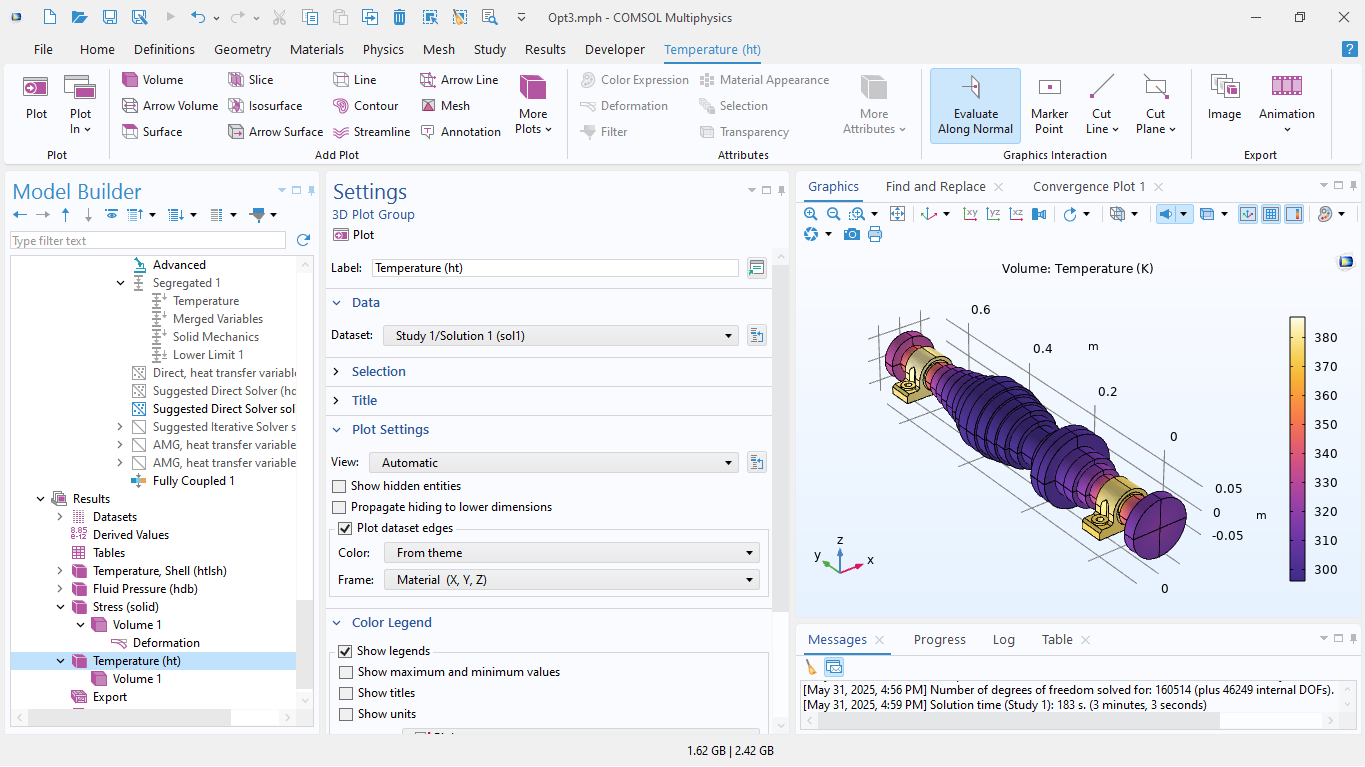
\includegraphics[width=0.9\textwidth]{temp_solidos.png}
              \caption{Temperatura en sólidos - Eje y cojinetes}
              \label{fig:comsol_temp_solidos_eje_cojinetes} % Etiqueta renombrada para mayor claridad
            \end{figure}

             \begin{figure}[H]
              \centering
              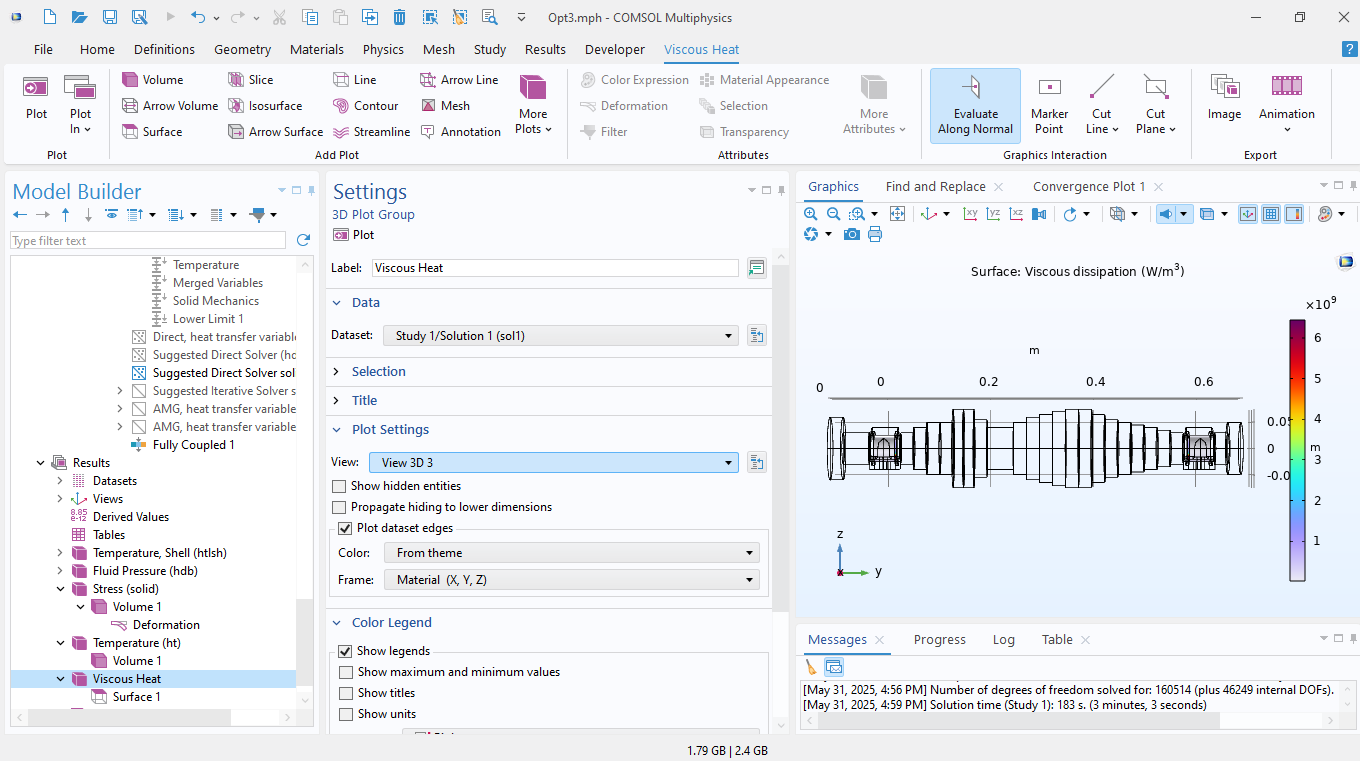
\includegraphics[width=0.9\textwidth]{visheat.png}
              \caption{Viscous Heat}
              \label{fig:comsol_viscous_heat} % Etiqueta renombrada para mayor claridad
            \end{figure}

            \begin{itemize}
              \item \textbf{Perfil de Temperatura:} La distribución de temperatura en el lubricante, el rotor y las carcasas muestra cómo el calor se disipa desde los rodamientos hacia el entorno. En los rodamientos, el calor se concentra donde la película de lubricante es más delgada.
              \item \textbf{Distribución de la Presión en los Rodamientos:} Se observó que la presión máxima se localiza en la parte inferior del rodamiento, lo cual es consistente con la teoría de que la mayor parte de la carga está soportada en esa región.
              \item \textbf{Tensiones Térmicas:} Las tensiones más altas se producen en el rotor, particularmente cerca de los rodamientos, debido a las restricciones térmicas impuestas por los cojinetes de empuje. La expansión térmica del rotor se ve limitada en estas zonas, creando tensiones axiales y radiales.
            \end{itemize}
          \section{Conclusiones}
La simulación ha demostrado que la disipación de calor en los rodamientos genera una distribución no uniforme de temperatura en el sistema, lo que provoca tensiones térmicas en el rotor y las carcasas.

La teoría sobre la disipación de calor por fricción del lubricante, junto con el modelo multiphysics implementado, ha permitido obtener una representación detallada del comportamiento térmico del sistema rotor-rodamiento. Estos resultados son cruciales para el diseño de sistemas rotativos,ayudando a prever posibles fallos debido a las tensiones térmicas en áreas críticas.
\bibliographystyle{apacite}
\nocite{*}
\bibliography{bib}
\end{document}